\chapter{Results}
This chapter reports the empirical performance of the three Linux translation implementations relative to a native Dual-Stack baseline in the three environments described in Chapter 4. The evaluation isolates the translation overhead of a CLAT-based path along two metrics: TCP throughput and ICMP round-trip time (RTT). Within each environment, comparisons are made relative to the IPv6 baseline to control for differences in virtualization and CPU topology across environments. Sections 5.1 and 5.2 present the throughput and RTT results, respectively. Sections 5.3 and 5.4 discuss the findings and document practical challenges.

\section{Throughput}
All throughput plots show time in seconds on the x-axis and throughput in Gbit/s on the y-axis and depict iperf3 time series over the configured measurement window. The AWS environment is considered first to set the stage for later changes in timing configuration and platform.
The initial AWS measurement run with the default kvm-clock shows a divergence in behavior between the user-space translators and Jool. Tayga and Tundra remain stable across repetitions, whereas both the native IPv6 baseline and Jool show large variability without a consistent trend. Since configuration, topology, and traffic generation were held constant, this pattern indicates platform caused timing artifacts rather than datapath specific instability. The clocksource was therefore assumed to be the primary source of variance, and following runs replaced kvm-clock with hpet to test this hypothesis. 

\begin{figure}[H]
    \centering
    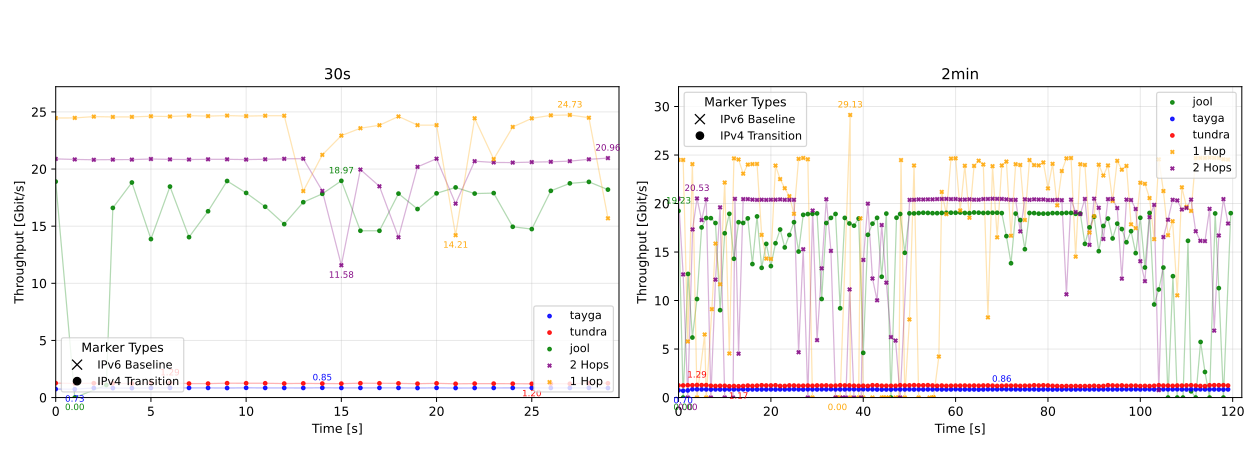
\includegraphics[width=1\textwidth]{resources/plots/CombinedPlot/TCP/AWS_tcp_sameScale_kvm-clock_linear.png}
    \caption{AWS cloud environment, KVM-clock, linear scale}
    \label{fig:AWS_tcp_sameScale_kvm-clock_linear}

\end{figure}
\begin{figure}[H]
    \centering
    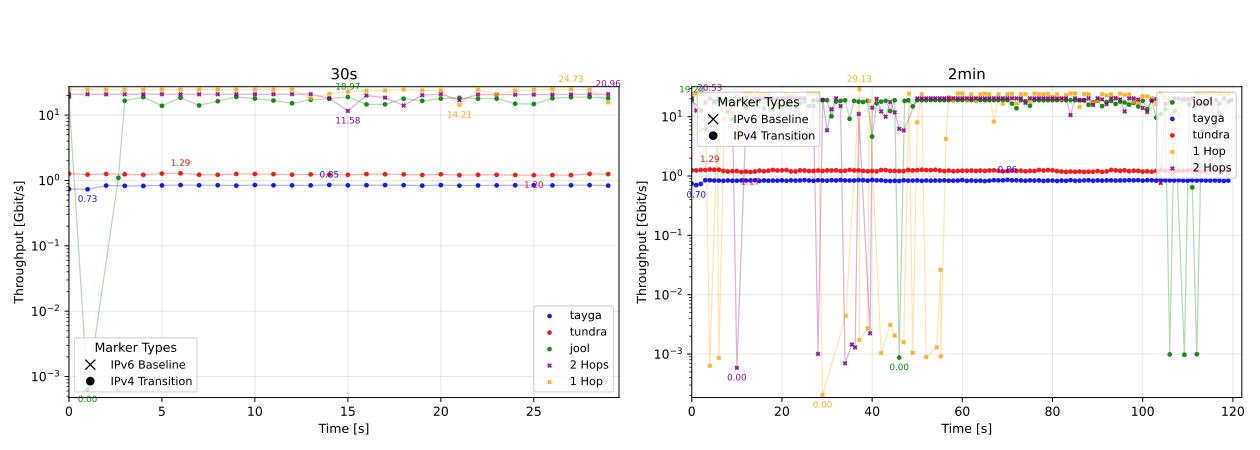
\includegraphics[width=1\textwidth]{resources/plots/CombinedPlot/TCP/AWS_tcp_sameScale_kvm-clock_log.png}
    \caption{AWS cloud environment, kvm-clock, logarithmic scale}
    \label{fig:AWS_tcp_sameScale_kvm-clock_log}

\end{figure}

Switching to hpet reduces anomalies but does not fully eliminate irregular throughput steps for the IPv6 baseline. Because the native baseline clusters near the top of the axis while the CLAT implementations cluster near the bottom, a dual-y-axis variant improves readability by separating the dynamic ranges without altering the underlying samples. The left y-axis scales the IPv6 baseline and the right y-axis scales the CLAT datapaths. Even here, the baseline still shows a step-like pattern, which is consistent with the remaining jitter. These results support the decision to move the same experimental topology to a local machine in order to reduce noise. 


\begin{figure}[H]
    \centering
    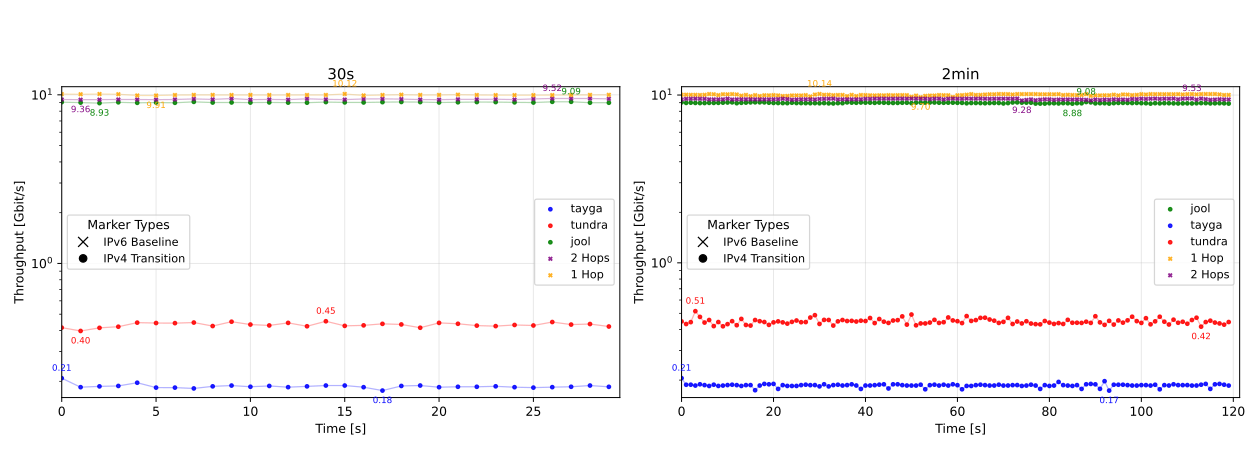
\includegraphics[width=1\textwidth]{resources/plots/CombinedPlot/TCP/AWS_tcp_sameScale_hpet_log.png}
    \caption{AWS cloud environment, hpet, log scale}
    \label{fig:AWS_tcp_sameScale_hpet_log}

\end{figure}


\begin{figure}[H]
    \centering
    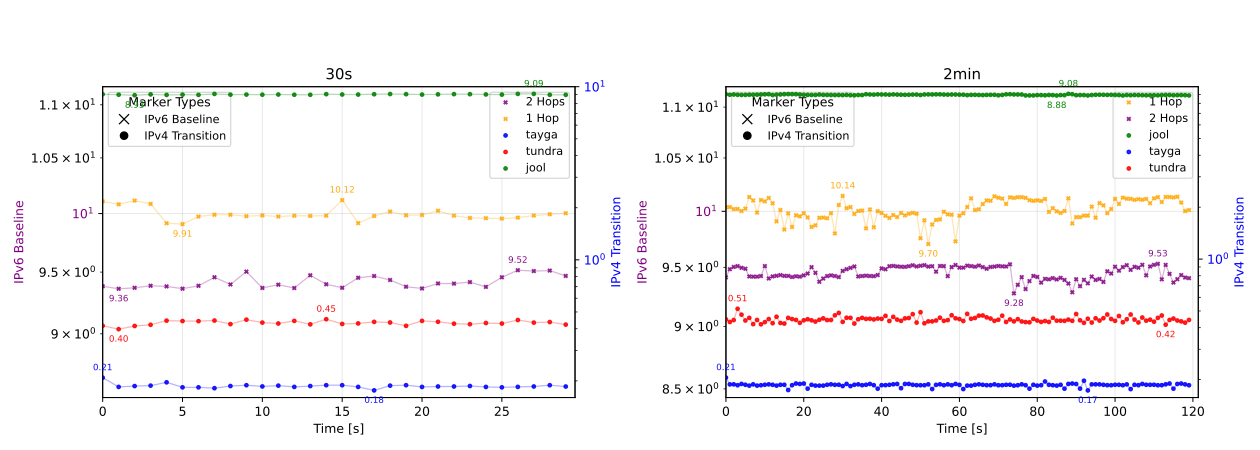
\includegraphics[width=1\textwidth]{resources/plots/JitterPlot/AWS_tcp_dualAxis_hpet_log.png}
    \caption{AWS Throughput Results, hpet, dual-y-axis, log scale}
    \label{fig:AWS_tcp_dualAxis_hpet_log}
\end{figure}



\paragraph{Local results}

On the single-host local machine, throughput stabilizes for both baseline and CLAT paths. The results show tight clustering across repetitions and a clear separation between one-hop and two-hop IPv6 baselines, consistent with the additional namespace traversal. Specifically, the one-hop baseline sustains approximately 41.61 Gbit/s, while the two-hop baseline sustains approximately 35.84 Gbit/s, which matches expectations for an extra hop. Within this environment, Jool consistently outperforms Tundra. Under TSC, Jool reaches a mean of about 33.7 Gbit/s versus 4.46 Gbit/s for Tundra. Under HPET, Jool's mean is about 6.735 Gbit/s versus 0.512 Gbit/s for Tundra. Tayga is not shown here due to the reasons summarized in Section 5.3. Because Tayga and Tundra are both stateless user-space translators with similar behavior, Tundra serves as a representative for this class in the single-host local setup, which is also in line with the AWS observations where Tayga and Tundra track closely.

\begin{figure}[H]
    \centering
    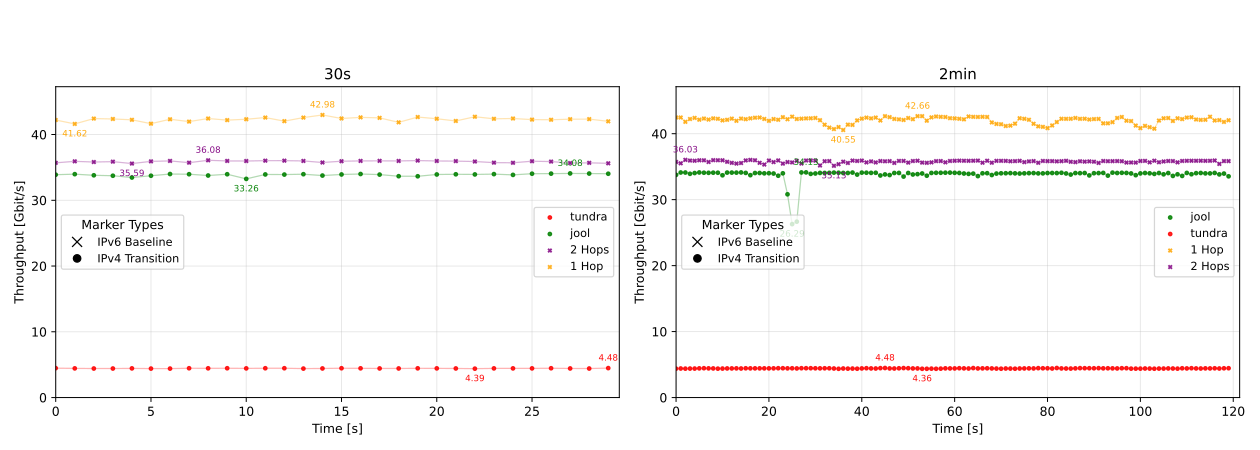
\includegraphics[width=1\textwidth]{resources/plots/CombinedPlot/TCP/Single_tcp_sameScale_tsc_linear.png}
    \caption{Single local machine, tsc, linear scale}
    \label{fig:Local_tcp_sameScale_tsc_linear}
\end{figure}

For consistency we also switched the clocksource to hpet in the local machine environment.

\begin{figure}[H]
    \centering
    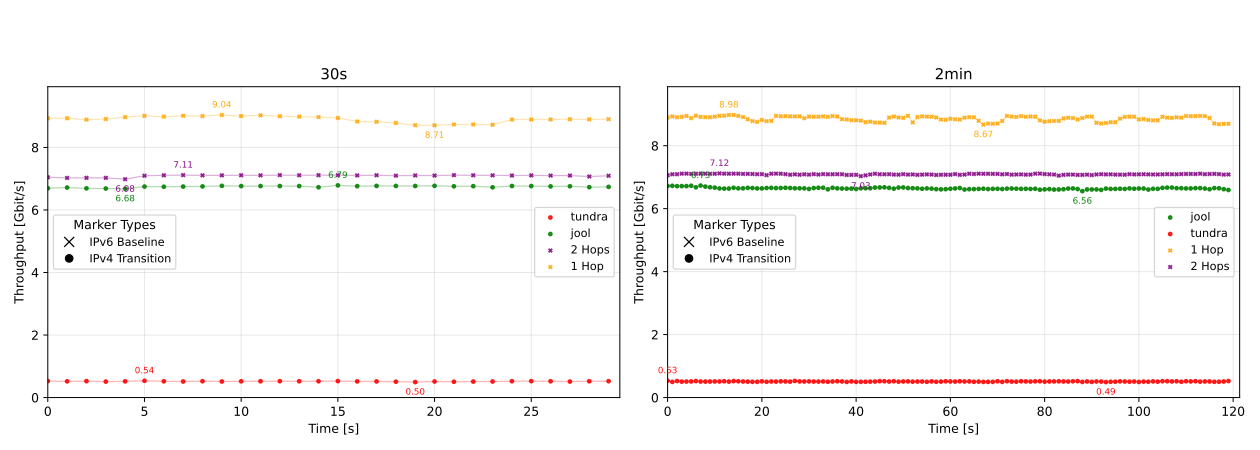
\includegraphics[width=1\textwidth]{resources/plots/CombinedPlot/TCP/Single_tcp_sameScale_hpet_linear.png}
    \caption{Single local machine, hpet, linear scale}
    \label{fig:Local_tcp_sameScale_hpet_linear}
\end{figure}

Figure \ref{fig:Local_tcp_dualAxis_hpet_linear} illustrates, in contrast to the earlier AWS dual-y-axis plot, a significantly more stable IPv6 baseline and a clear distinction between the two CLAT implementations.

\begin{figure}[H]
    \centering
    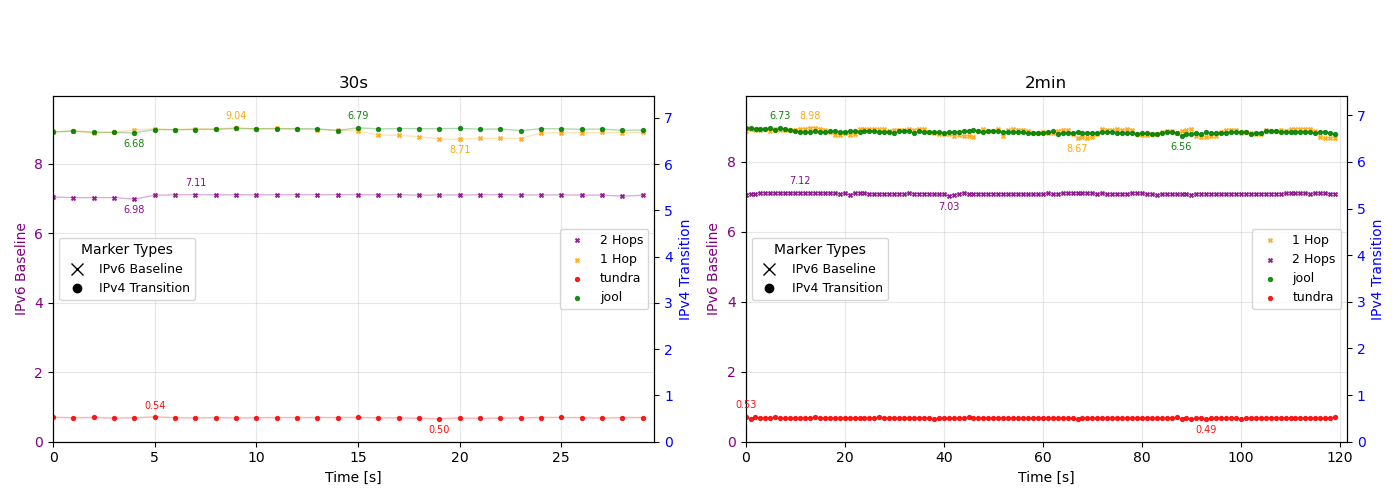
\includegraphics[width=1\textwidth]{resources/plots/JitterPlot/Single_tcp_dualAxis_hpet_linear.png}
    \caption{Single local machine, hpet, dual-y-axis, linear scale}
    \label{fig:Local_tcp_dualAxis_hpet_linear}
\end{figure}



The dual-host local setup introduces a physical 1 Gbit/s Ethernet link that caps the achievable throughput for all datapaths. In this environment, the absolute advantage of the kernel-space datapath on loopback is compressed by the link bottleneck, and both Jool and Tundra approach the capacity limit. Jool peaks near 0.66 Gbit/s while Tundra approaches 0.57 Gbit/s and the IPv6 baselines are bounded by 1 Gbit/s as expected under both TSC and HPET. The slight upward trends over time are caused by TCP congestion control behavior but does not affect the ordering of the results. The key observation is that when the bottleneck is the external link rather than the host datapath, the differences between CLAT implementations become small relative to the link capacity, and the gap to the dual-stack baseline largely disappears.


\begin{figure}[H]
    \centering
    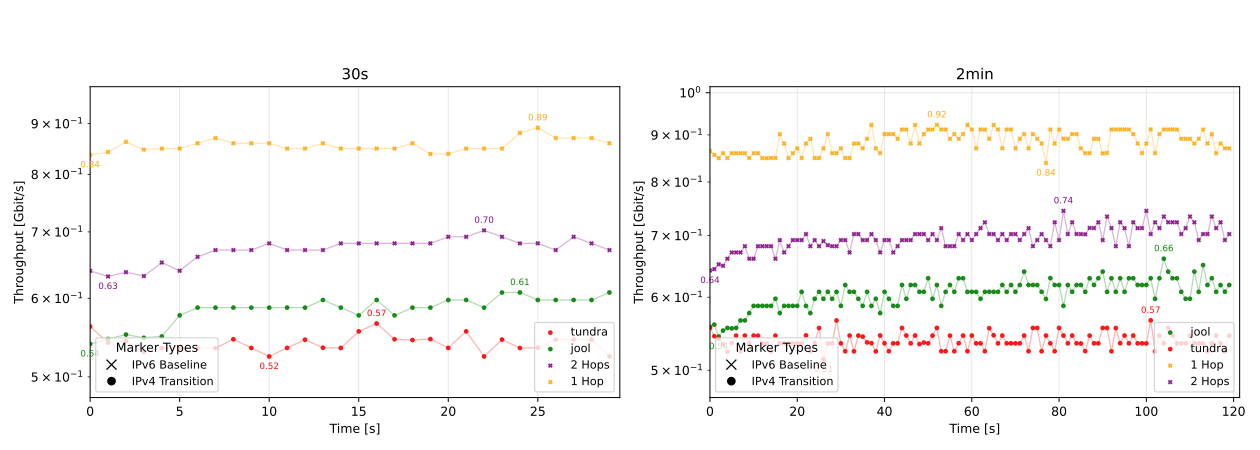
\includegraphics[width=1\textwidth]{resources/plots/CombinedPlot/TCP/Double_tcp_sameScale_hpet_log.png}
    \caption{Dual local machines, hpet, log scale}
    \label{fig:Dual_tcp_sameScale_hpet_log}
\end{figure}

\begin{figure}[H]
    \centering
    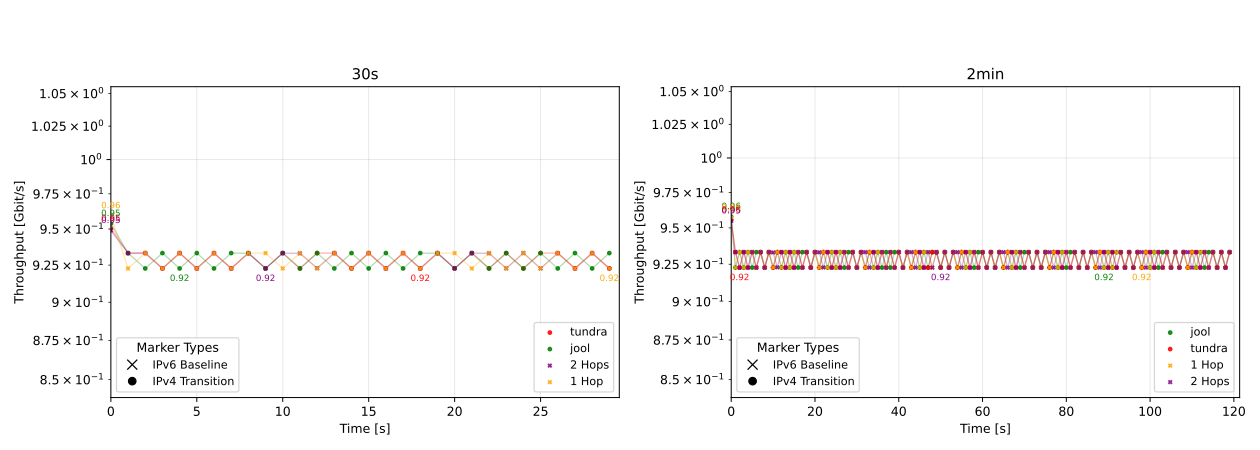
\includegraphics[width=1\textwidth]{resources/plots/CombinedPlot/TCP/Double_tcp_sameScale_tsc_log.png}
    \caption{Dual local machines, tsc, log scale}
    \label{fig:Dual_tcp_sameScale_tsc_log}
\end{figure}

Looking at the dual-y-axis plot in Figure \ref{fig:Double_tcp_dualAxis_hpet_log} for this scenario, the IPv6 baseline shows a stable throughput compared to the AWS environment.
\begin{figure}[H]
    \centering
    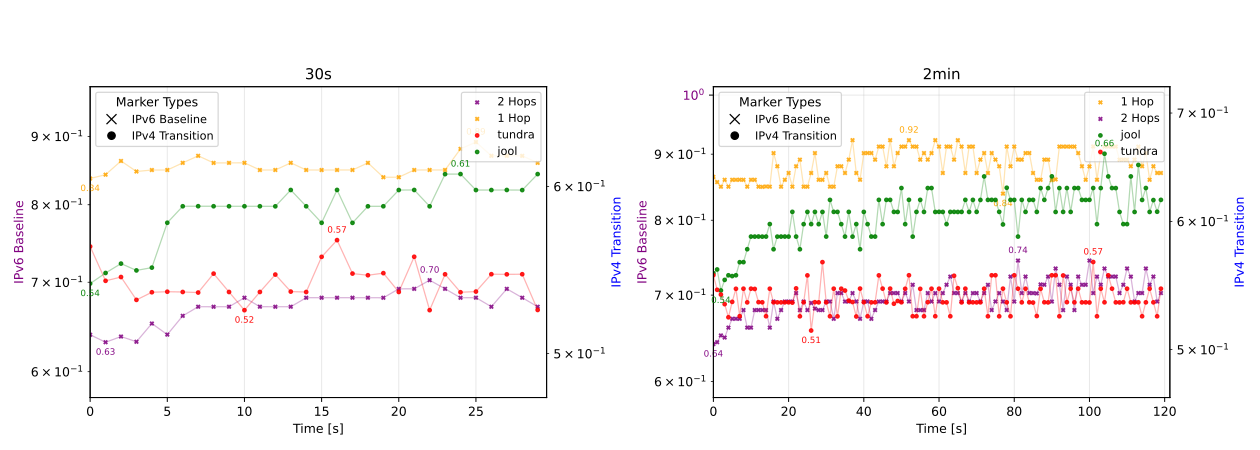
\includegraphics[width=1\textwidth]{resources/plots/JitterPlot/Double_tcp_dualAxis_hpet_log.png}
    \caption{Single local machine, hpet, dual-y-axis, log scale}
    \label{fig:Double_tcp_dualAxis_hpet_log}
\end{figure}

Across environments, two effects stand out. First, the translation overhead of CLAT relative to a native IPv6 baseline is strongly environment-dependent. On loopback, Jool’s kernel datapath yields a substantial advantage over user-space due to fewer context switches and reduced packet copy overhead, while on a 1 Gbit/s physical link the advantage compresses toward the link limit. Second, clocksource selection has a measurable impact on time series smoothness and on the dispersion of repeated measurements, especially under virtualization. The local machine results show that platform-induced jitter can dominate differences in the cloud.

\section{RTT}
The RTT results mirror the throughput analysis in showing that the translation cost is small and that kernel-space translation retains a consistent advantage over user-space, while environment and topology shape absolute values. In the AWS environment under HPET, a clear gap separates the IPv6 baselines from the CLAT datapaths, consistent with the expectation that translation introduces additional per-packet processing. The one hop IPv6 baseline centers around 0.045 ms and the two hop baseline around 0.052 ms. Among translators, Jool achieves a mean of approximately 0.065 ms, while Tayga and Tundra lie around 0.086 ms and 0.095 ms, respectively. The relative ordering is therefore consistent with the throughput results. 


\begin{figure}[H]
    \centering
    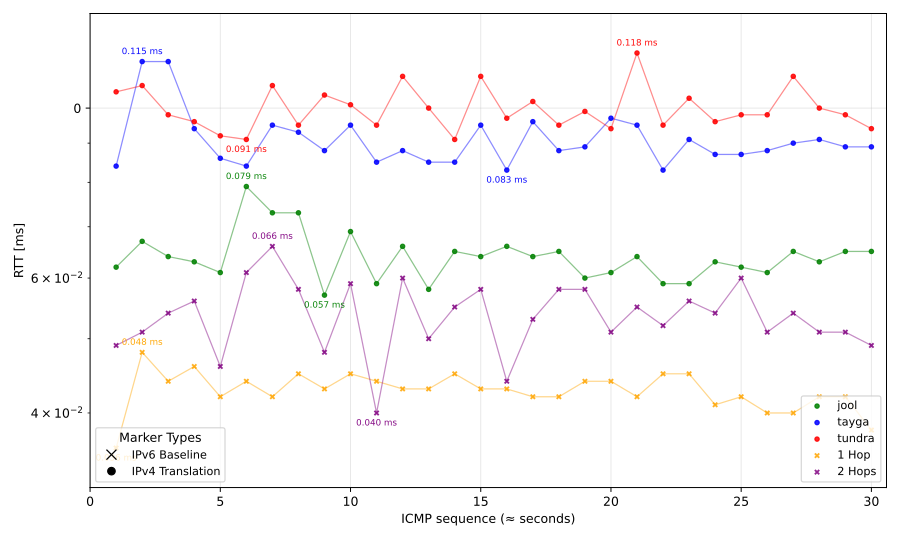
\includegraphics[width=1\textwidth]{resources/plots/CombinedPlot/RTT/AWS_ping_rtt_Ping_30s_log.png}
    \caption{AWS cloud environment, hpet, log scale}
    \label{fig:AWS_icmp_sameScale_hpet_log}

\end{figure}

On the single host local machine, RTTs increase across all datapaths relative to AWS, which is explained by the host’s lower CPU performance. The ordering remains unchanged: Jool again exhibits the lowest CLAT latency with a mean of about 0.182 ms, while Tundra’s mean is around 0.25 ms. The spread within each series is narrower than in AWS, consistent with the reduced timing jitter observed for throughput. 

\begin{figure}[H]
    \centering
    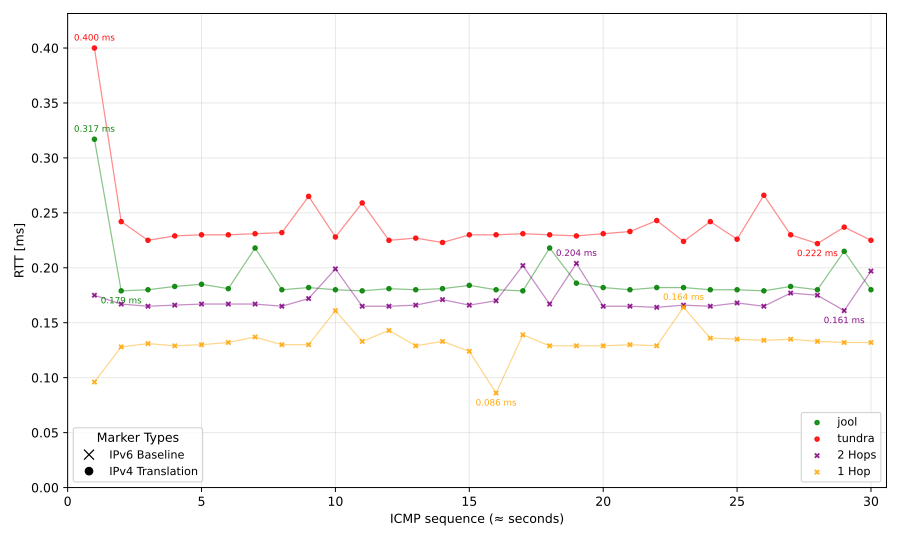
\includegraphics[width=1\textwidth]{resources/plots/CombinedPlot/RTT/Single_ping_rtt_Ping_30s_linear.png}
    \caption{Single local machine environment, hpet, linear scale}
    \label{fig:Local_icmp_sameScale_hpet_linear}
\end{figure}

The dual-host local setup produces the highest RTTs due to the additional physical hop traversing the Ethernet link. Variability increases across all datapaths, reflecting the added queueing opportunities along the path. Despite the shift in absolute values, the relative ordering persists, with Jool maintaining a modest latency advantage over user-space translation. The gap to the IPv6 baselines remains small in absolute terms, which supports the thesis that CLAT overhead is limited in practice. 


\begin{figure}[H]
    \centering
    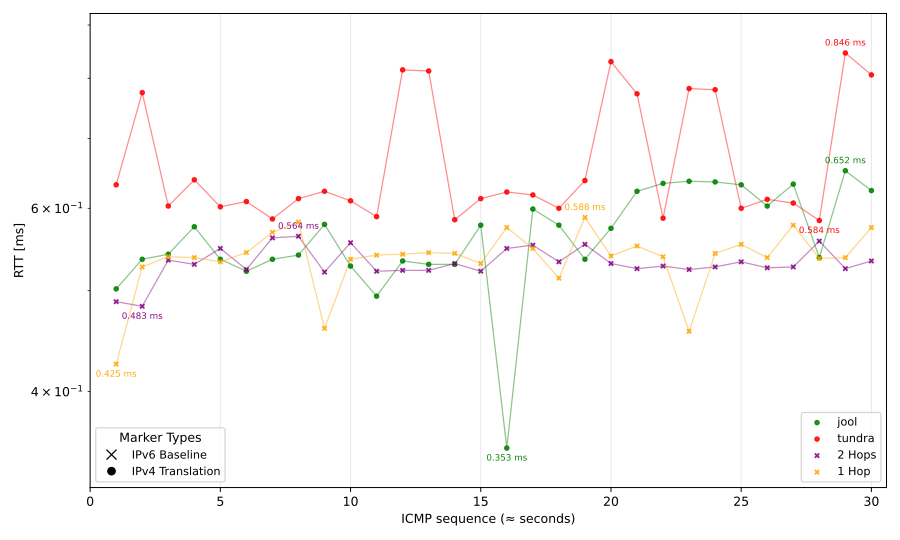
\includegraphics[width=1\textwidth]{resources/plots/CombinedPlot/RTT/Double_ping_rtt_Ping_30s_log.png}
    \caption{Dual local machines environment, hpet, log scale}
    \label{fig:Dual_icmp_sameScale_hpet_log}
\end{figure}



\section{Discussion}

\section{Challenges and Solutions}